\section{Alta, baja y modificación de datos (ABMs)}
En esta sección explicamos como realizar el alta, baja y modificación de datos del sistema, es decir, síntomas, discriminantes y usuarios.

\subsection{Acceso al menú de configuración}
Para poder acceder al menú de configuración de datos, el usuario actual debe tener el rol de administrador. En caso contrario dicho menú permanecerá oculto (ver figuras \ref{fig:menu_conf_visible} y \ref{fig:menu_conf_oculto}).

\begin{figure}
\centerline{
\includegraphics[width=0.7\textwidth]{menu_configuracion_visible.png}}
\caption{Menú de configuración visible}
\label{fig:menu_conf_visible}
\end{figure}

\begin{figure}
\centerline{
\includegraphics[width=0.7\textwidth]{menu_configuracion_oculto.png}}
\caption{Menú de configuración oculto}
\label{fig:menu_conf_oculto}
\end{figure}

\subsection{ABM de síntomas}
Para acceder a la pantalla de administración de síntomas nos dirigimos hacia ``Configuración'' y luego a ``Síntomas'' (ver figura \ref{fig:menu_sintomas}).
\begin{figure}
\centerline{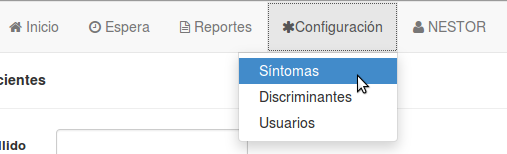
\includegraphics[width=0.7\textwidth]{menu_sintomas.png}}
\caption{Menú de síntomas}
\label{fig:menu_sintomas}
\end{figure}
Allí se nos muestra el listado de todos los síntomas cargados en el sistema (figura \ref{fig:listado_sintomas}).

\begin{figure}
\centerline{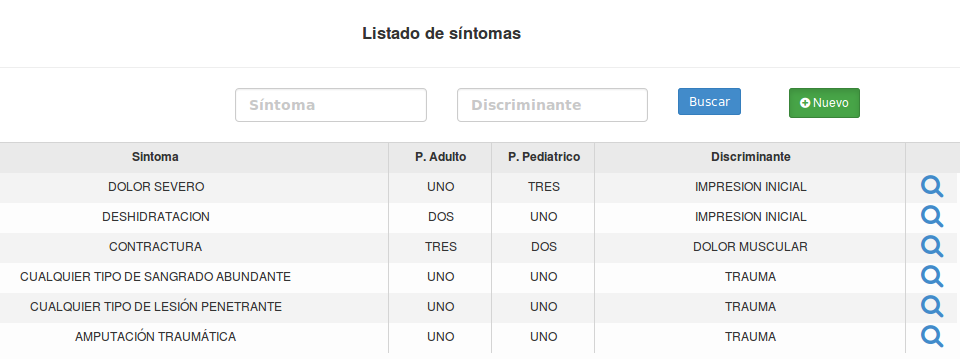
\includegraphics[width=1\textwidth]{listado_sintomas.png}}
\caption{Listado de síntomas}
\label{fig:listado_sintomas}
\end{figure}

\subsubsection{Alta de síntoma}\label{cap:alta_sintoma}
Para dar de alta un nuevo síntoma hacemos click en el botón ``Nuevo'', en la pantalla del listado de síntomas, que nos dirige a la pantalla del detalle del síntoma (figura \ref{fig:detalle_sintoma}).
\begin{figure}
\centerline{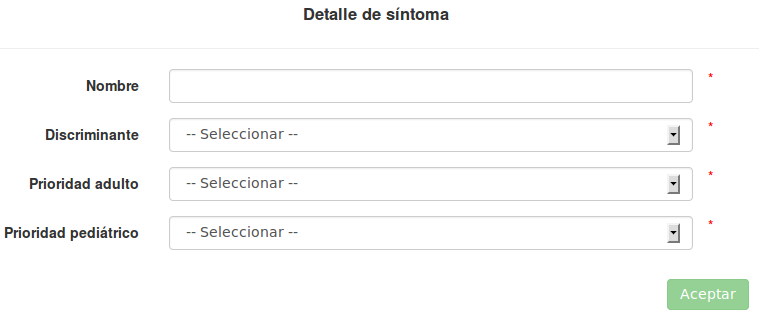
\includegraphics[width=1\textwidth]{detalle_sintoma.png}}
\caption{Detalle de síntoma}
\label{fig:detalle_sintoma}
\end{figure}
Allí debemos ingresar el nombre, el discriminante, la prioridad para adultos y la prioridad para pediátricos. Tener en cuenta que si el discriminante que deseamos no aparece en el listado desplegable entonces primero debemos darle de alta como explicaremos en la sección \ref{cap:alta_discriminante}). Luego de llenar todos los campos, el botón ``Aceptar'' se desbloquea y si le hacemos click aparece un mensaje que confirma que el síntoma fue ingresado con éxito (figura \ref{fig:sintoma_cargado_con_exito}).
\begin{figure}
\centerline{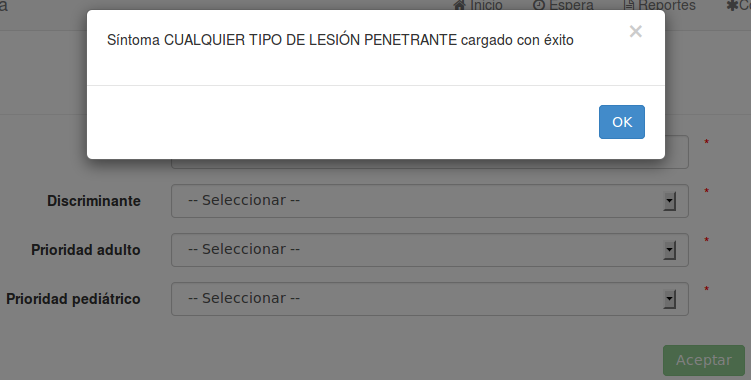
\includegraphics[width=1\textwidth]{sintoma_cargado_con_exito.png}}
\caption{Mensaje de síntoma cargado con éxito}
\label{fig:sintoma_cargado_con_exito}
\end{figure}

\subsubsection{Modificación de síntoma}\label{cap:modificacion_sintoma}
Para modificar un síntoma que hayamos dado de alta con anterioridad debemos seleccionarlo del listado de síntomas. Para facilitar la búsqueda del mismo podemos filtrar el listado llenando los campos de ``Síntoma'' y/o ``Discriminante'' (ver sección \ref{cap:filtrado_listado}). Si encontramos el síntoma buscado hacemos click en el botón ``Ver detalle''(ver figura \ref{fig:sintomas_filtro}) 
\begin{figure}
\centerline{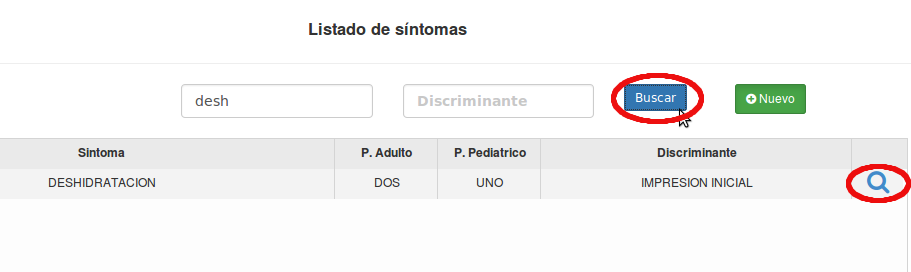
\includegraphics[width=1\textwidth]{sintomas_listado_buscar.png}}
\caption{Listado de síntomas filtrado. Aparecen los botones ``Buscar'' y ``Ver detalle'' señalados en rojo}
\label{fig:sintomas_filtro}
\end{figure}
que nos lleva a la pantalla de ``Detalle de síntoma'' con todos los campos cargados. Allí podemos modificar los valores que deseemos y al apretar ``Aceptar'' aparece el mensaje de confirmación de síntoma actualizado con éxito (figura \ref{fig:sintoma_actualizado_con_exito}).
\begin{figure}
\centerline{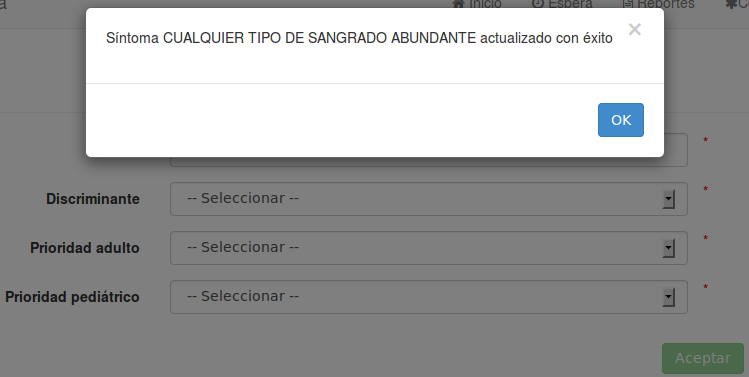
\includegraphics[width=1\textwidth]{sintoma_actualizado_con_exito.png}}
\caption{Mensaje de confirmación de síntoma actualizado con éxito}
\label{fig:sintoma_actualizado_con_exito}
\end{figure}

\subsubsection{Baja de síntoma}
Una vez creados, los síntomas no se pueden eliminar. Solo se pueden modificar como explicamos en la sección anterior. Lo mismo sucede con los discriminantes de síntomas.

\subsection{ABM de discriminantes de síntomas}\label{ABM_discriminantes}
Para acceder a la pantalla de administración de discriminantes de síntomas nos dirigimos hacia ``Configuración'' y luego a ``Discriminantes'' (ver figura \ref{fig:menu_discriminantes}).
\begin{figure}
\centerline{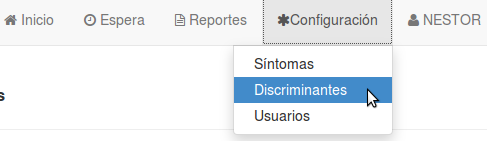
\includegraphics[width=0.7\textwidth]{menu_discriminantes.png}}
\caption{Menú de discriminantes de síntomas}
\label{fig:menu_discriminantes}
\end{figure}
Allí se nos muestra el listado de todos los discriminantes de síntomas cargados en el sistema (figura \ref{fig:listado_discriminantes}).
\begin{figure}
\centerline{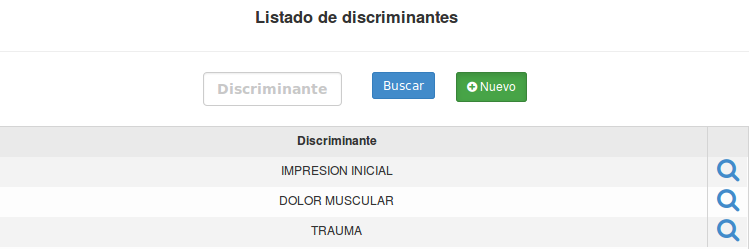
\includegraphics[width=1\textwidth]{listado_discriminantes.png}}
\caption{Listado de discriminantes de síntomas}
\label{fig:listado_discriminantes}
\end{figure}

\subsubsection{Alta de discriminante de síntoma}\label{cap:alta_discriminante}
Para dar de alta un nuevo discriminante de síntoma hacemos click en el botón ``Nuevo'', en la pantalla del listado de discriminantes de síntomas, que nos dirige a la pantalla de alta de discriminante (figura \ref{fig:nuevo_discriminante}).
\begin{figure}
\centerline{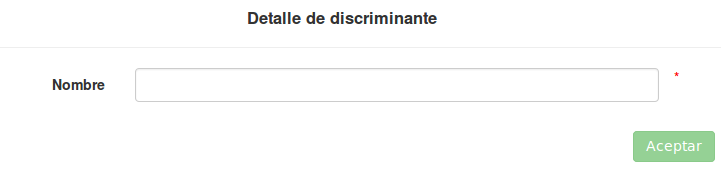
\includegraphics[width=1\textwidth]{nuevo_discriminante.png}}
\caption{Alta de discriminante de síntoma}
\label{fig:nuevo_discriminante}
\end{figure}
Allí debemos ingresar el nombre del discriminante, lo que desbloquea el botón ``Aceptar'' y si le hacemos click aparece un mensaje que confirma que el discrimnante fue ingresado con éxito. Una vez cargado el discriminante podremos ingresar nuevos síntomas de ese discriminante, como explicamos anteriormente en la sección \ref{cap:alta_sintoma}.

\subsubsection{Modificación de un discriminante de síntoma}
Para modificar el nombre de un discriminante de síntoma debemos seleccionarlo del listado de discriminantes\footnote{Por cuestiones de lógica del Triage podemos modificar cualquier discriminante a excepción de ``IMPRESIÓN INICIAL''.}. Para facilitar la búsqueda del mismo podemos filtrar el listado llenando el campo ``Discriminante'' (ver sección \ref{cap:filtrado_listado}). Si encontramos el discriminante buscado hacemos click en el botón ``Ver detalle'' que nos lleva a la pantalla de ``Detalle de discriminante'' con el campo ``Nombre'' cargado y con un listado que nos muestra todos los síntomas de ese discriminante (ver figura \ref{fig:detalle_discriminante}).
\begin{figure}
\centerline{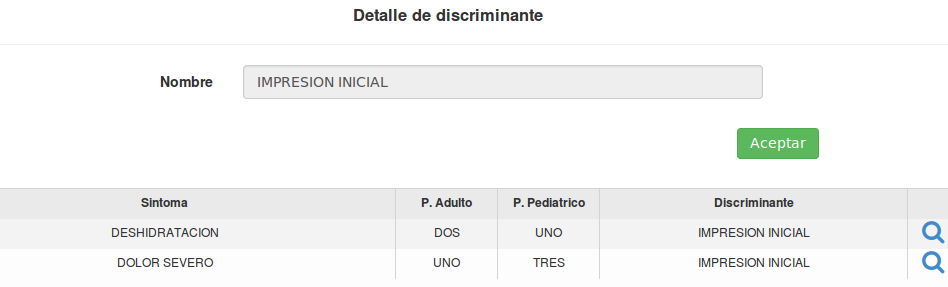
\includegraphics[width=1\textwidth]{listado_sintomas_de_discriminante.png}}
\caption{Detalle del discriminante con listado de síntomas}
\label{fig:detalle_discriminante}
\end{figure}
En esa pantalla podemos modificar el nombre del discriminante y al apretar ``Aceptar'' aparece el mensaje de confirmación de discriminante actualizado con éxito. También podemos hacer click en el botón ``Ver detalle'' de algún síntoma del listado para ir a la pantalla de ``Detalle de síntoma'' y modificarlo como mostramos anteriormente en la sección \ref{cap:modificacion_sintoma}.

\subsubsection{Baja de discriminante de síntoma}
Al igual que los síntomas, una vez creados, los discriminantes de síntomas no se pueden eliminar. Solo podemos modificarles el nombre como explicamos en la sección anterior.